\documentclass[
  captions=tableheading,
  bibliography=totoc, 
  titepage=firstiscover,
]{scrartcl}

\usepackage{blindtext} %neuer input

\usepackage{longtable} % Tabellen über mehrere Seiten

\usepackage[utf8]{inputenc} %neuer input

\usepackage{scrhack}

\usepackage[aux]{rerunfilecheck} %Warnung falls nochmal kompiliert werden muss

\usepackage{fontspec} %Fonteinstellungen

\recalctypearea{}

\usepackage[main=ngerman]{babel} %deutsche Spracheinstellung

\usepackage{ragged2e} %neuer input

\usepackage{amsmath, nccmath}

\usepackage{amssymb} %viele mathe Symbole

\usepackage{mathtools} %Erweiterungen für amsmath


\DeclarePairedDelimiter{\abs}{\lvert}{\rvert}
\DeclarePairedDelimiter{\norm}{\lVert}{\rVert}

\DeclarePairedDelimiter{\bra}{\langle}{\rvert}
\DeclarePairedDelimiter{\ket}{\lvert}{\rangle}

\DeclarePairedDelimiterX{\braket}[2]{\langle}{\rangle}{
#1 \delimsize| #2
}

\NewDocumentCommand \dif {m}
{
\mathinner{\symup{d} #1}
}


\usepackage[
  math-style=ISO,
  bold-style=ISO,
  sans-style=italic,
  nabla=upright,
  partial=upright,
  warnings-off={
    mathtools-colon,
    mathtools-overbracket,
  },
]{unicode-math}

\setmathfont{Latin Modern Math}
\setmathfont{XITS Math}[range={scr, bfscr}]
\setmathfont{XITS Math}[range={cal, bfcal}, StylisticSet=1]


\usepackage[
  locale=DE,
  separate-uncertainty=true,
  per-mode=reciprocal,
  output-decimal-marker={,},
]{siunitx}

\usepackage[autostyle]{csquotes} %richtige Anführungszeichen

\usepackage{xfrac}

\usepackage{float}

\floatplacement{figure}{htbp}

\floatplacement{table}{htbp}

\usepackage[ %floats innerhalb einer section halten
  section,   %floats innerhalb er section halten
  below,     %unterhalb der Section aber auf der selben Seite ist ok
]{placeins}

\usepackage[
  labelfont=bf,
  font=small,
  width=0.9\textwidth,
]{caption}

\usepackage{subcaption} %subfigure, subtable, subref

\usepackage{graphicx}

\usepackage{grffile}

\usepackage{booktabs}

\usepackage{microtype} %Verbesserungen am Schriftbild

\usepackage[
backend=biber,
]{biblatex}

\addbibresource{../lit.bib}

\usepackage[ %Hyperlinks im Dokument
  german,
  unicode,
  pdfusetitle,
  pdfcreator={},
  pdfproducer={},
]{hyperref}

\usepackage{bookmark}

\usepackage[shortcuts]{extdash}

%\usepackage{warpcol}


\begin{document}
    \title{V303 Lock-In-Verstärker}
    \author{  
    Tobias Rücker\\
    \texorpdfstring{\href{mailto:tobias.ruecker@tu-dortmund.de}{tobias.ruecker@tu-dortmund.de}
    \and}{,} 
    Paul Störbrock\\
    \texorpdfstring{\href{mailto:paul.stoerbrock@tu-dortmund.de}{paul.stoerbrock@tu-dortmund.de}}{}
    }
    \date{Durchführung:14.01.2020 , Abgabe:21.01.2020  \vspace{-4ex}}
\maketitle
\center{\Large Versuchsgruppe: \textbf{42}}
\thispagestyle{empty}

\newpage
\tableofcontents
\thispagestyle{empty}
\newpage

% Ziel %%%%%%%%%%%%%%%%%%%%%%%%%%%%%%%%%%%%%%%%%%%%%%%%%%%%%%%%%%%%%%%%%%%%%%%%%%%%%%%%%%%%%%%%%%%%%%%%%%%%%%%%%%%%%%%%%%%%%%%%%%%%%%%%%%%%%%%%%%%%%%%%%%%%%%%%%%%%%%%%%%%%%%%%%%%%%%%%%%%%%%%%%%%%%%%%%%%%%%%%%%%%%%%%%

\setcounter{page}{1}
\section{Ziel}\justifying
Bei Messungen von Signalen sind diese häufig durch die Hintergrundstrahlung stark verrauscht. 
Der Lock-In-Verstärker löst dieses Problem und filtert das Messsignal aus dem rauschen
heraus. Daher wird sich die Funktionsweise dieses Verstärkers näher betrachtet.

% Theorie %%%%%%%%%%%%%%%%%%%%%%%%%%%%%%%%%%%%%%%%%%%%%%%%%%%%%%%%%%%%%%%%%%%%%%%%%%%%%%%%%%%%%%%%%%%%%%%%%%%%%%%%%%%%%%%%%%%%%%%%%%%%%%%%%%%%%%%%%%%%%%%%%%%%%%%%%%%%%%%%%%%%%%%%%%%%%%%%%%%%%%%%%%%%%%%%%%

\section{Theorie}\justifying
Bei einem Lock-In-Verstärker wird ein verrauschtes Signal durc einen Bannpass geleitet.
Ein Bannpass stellt eine elektrische Schaltung dar, welches einen bestimmten 
Frequenzbereich aus einem Signal herausfiltert. Das, vom Phasenschieber variierte, 
Referenzsignal mit der Frequenz $\omega _0$ wird vom Mischer mit dem Signal multipliziert.
Dannach wird das daraus entstehende durch einen Tiefpassfilter geleitet. der Tiefpassfilter
integriert dabei für $\tau =RC \gg \sfrac{1}{\omega _0} $ das Mischsignal.
Durch den Tiefpass wird bei großem $\tau$ die Bandbreite des Rauschens beliebig klein.
Durch den Tiefpassfilter ergibt sich für ein um $phi$ phasenverschobenes 
Referenzsignal eine Ausgangnsspannung in der Forms
\begin{align}
    U_{\text{out}}= \frac{2}{\pi} U_0 \cos{\Phi}
\end{align}
% Fehlerrechnung %%%%%%%%%%%%%%%%%%%%%%%%%%%%%%%%%%%%%%%%%%%%%%%%%%%%%%%%%%%%%%%%%%%%%%%%%%%%%%%%%%%%%%%%%%%%%%%%%%%%%%%%%%%%%%%%%%%%%%%%%%%%%%%%%%%%%%%%%%%%%%%%%%%%%%%%%%%%%%%%%%%%%%%%%%%%%%%%%%%%%%%%%%%%%%%%%%%%%%

\section{Fehlerrechnung}\justifying

Für die Berechnung von Messunsicherheiten werden in diesem Protokoll folgende Formeln
verwendet:
\begin{subequations} \label{eq:}
\begin{align} 
\intertext{Zur Bestimmung eines Mittelwertes wird folgende Formel benutzt:
}
    \overline{x} &= \frac{1}{N}\sum_{i=1}^{N} x_i \label{eq:a}
\intertext{Zur Bestimmung der Messunsicherheit bei Mittelwerten wird mit der Formel
}
    \Delta\overline{x} &= \frac{1}{\sqrt{N}} \sqrt{\frac{1}{1-N} \sum_{i=1}^{N} (x_i - \overline{x})^2} \label{eq:b},
\intertext{gearbeitet und die Gaußsche Fehlerfortpflanzung wird mit
}
    \Delta f &= \sqrt{\sum_{i=1}^{N} \left( \frac{\delta f}{\delta x_i} \right)^2 \cdot (\Delta x_i)^2} \label{eq:c}
\intertext{berechnet. Um Ausgleichsgeraden und ihre Parameter zu bestimmen, werden folgende Formeln verwendet:
}
    y &= m \cdot x + b \label{eq:6d} \\ 
    m &= \frac{\overline{xy} - \overline{x} \cdot \overline{y}}{\overline{x^2} - {\overline{x}}^2} \label{eq:e}\\
    b &= \frac{\overline{y} \cdot \overline{x^2} - \overline{xy} \cdot \overline{x}}{\overline{x^2} - {\overline{x}}^2} \label{eq:f}
\end{align}
\end{subequations}

% Versuchsaufbau + Versuchsdurchführung %%%%%%%%%%%%%%%%%%%%%%%%%%%%%%%%%%%%%%%%%%%%%%%%%%%%%%%%%%%%%%%%%%%%%%%%%%%%%%%%%%%%%%%%%%%%%%%%%%%%%%%%%%%%%%%%%%%%%%%%%%%%%%%%%%%%%%%%%%%%%%%%%%%%%%%%%%%%%%%%%%%%%%%%%%%%%%%%%%%%%%%%%%%%%%%%%%

\section{Versuchsaufbau und Versuchsdurchführung}\justifying

\flushleft{Benötigt\;}\justifying werden: \textit{Ein Lock-In-Verstärker, ein Digitales Oszilloskop, acht BNC Verbindungskabel, eine BNC 
Steckverbindung, ein USB Stick, eine Leuchtdiode (LED), ein Photodetektor und eine Skala (ca. $\SI{50}{\centi\meter}$).}

\flushleft{Zuerst\;}\justifying wird das ungestörte Signal $U_{sig}$ und das Referenzsignal $U_{ref}$, welche vom Reference/Oscillator ausgegeben werden, 
vom Oszilloskop abgebildet. Damit wird das variable Signal bestimmt. Nachdem das variable Signal gefunden wurde, wird dem Oszilloskop die Amplitude 
des konstanten Signals entnommen. 

\flushleft{Anschließend\;}\justifying wird der Versuch, wie in der folgenden Abbildung \ref{fig:1} dargestellt, aufgebaut: 

\begin{figure}[H]
    \centering
    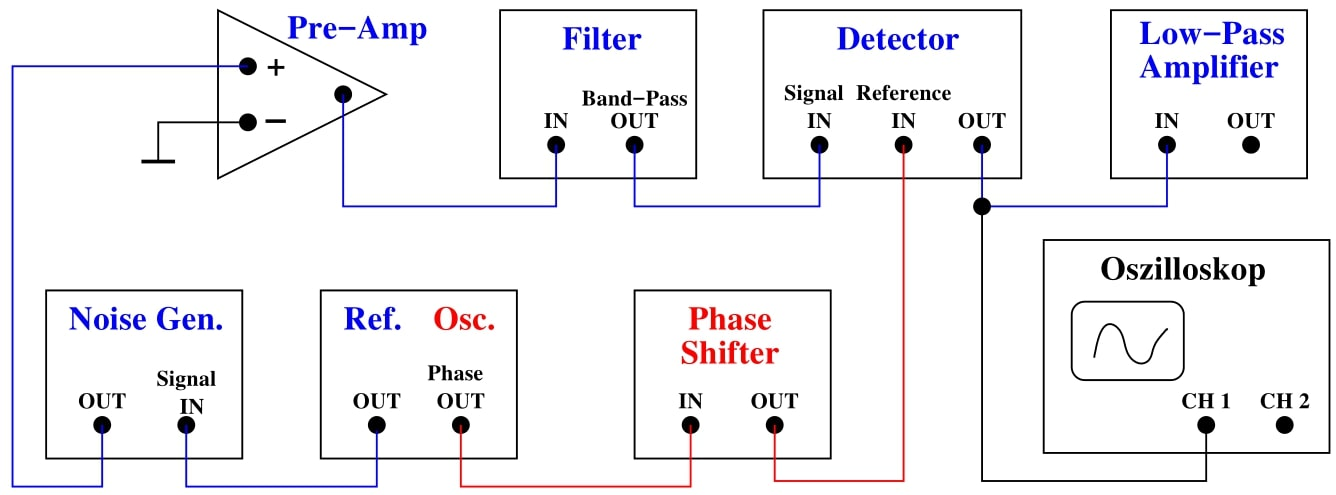
\includegraphics[width=\linewidth]{./images/lock-in.jpg}
    \caption{Versuchsaufbau des Lock-In-Verstärkers \cite{V303}}
    \label{fig:1}
\end{figure}

\flushleft{Zunächst\;}\justifying wird der Noise Generator überbrückt, damit das ungestörte Signal $U_{sig}$ mit dem Referenzsignal $U_{ref}$
im Detector gemischt werden kann. Anschließend wird der USB Stick am Oszilloskop angeschlossen und es werden für zehn Phasen das Phasendiagramm 
der gemischten Signale gespeichert.

\flushleft{Nun\;}\justifying wird der Noise Generator dazu geschaltet. Für das nun gestörte Signal $U_{sig}$ werden erneut Messungen für zehn Phasen 
durchgeführt. 

\flushleft{Anschließend\;}\justifying wird der Aufbau wie in Abbildung \ref{fig:2} abgeändert, sodass nun eine LED und ein Photodetektor den 
Noise Generator ersetzen:

\begin{figure}[H]
    \centering
    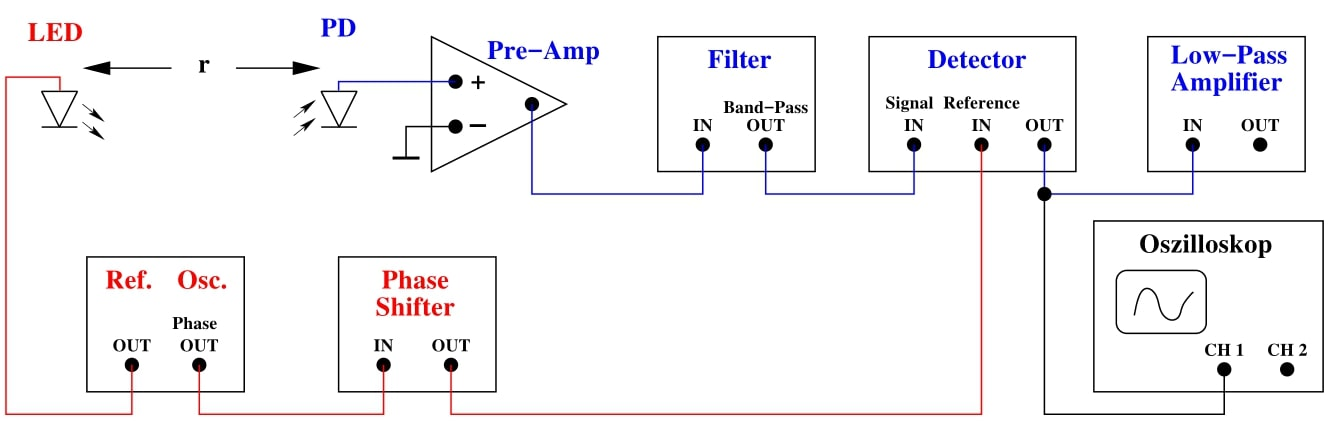
\includegraphics[width=\linewidth]{./images/lock-in_led.jpg}
    \caption{Versuchsaufbau des Lock-In-Verstärkers mit LED \cite{V303}}
    \label{fig:2}
\end{figure}

\flushleft{Die\;}\justifying LED  und der Photodetektor werden auf einer Skala montiert, dabei soll die LED beweglich bleiben und der Detector stationär.
Die LED soll einer Leuchtfrequenz zwischen $\SI{50}{\hertz}$ und $\SI{500}{\hertz}$ zugewiesen werden. Nun wird die LED um gleichmäßige Distanzen
von dem Photodetektor wegbewegt, hier um $\SI{2}{\centi\meter}$. Für jede neue Distanz wird die Intensität am Oszilloskop abgelesen. Sobald sich keine
Änderung der Intensität am Oszilloskop erkennen lässt, werden keine weiteren Messwerte mehr aufgenommen.  

% Auswertung %%%%%%%%%%%%%%%%%%%%%%%%%%%%%%%%%%%%%%%%%%%%%%%%%%%%%%%%%%%%%%%%%%%%%%%%%%%%%%%%%%%%%%%%%%%%%%%%%%%%%%%%%%%%%%%%%%%%%%%%%%%%%%%%%%%%%%%%%%%%%%%%%%%%%%%%%%%%%%%%%%%%%%%%%%%%%%%%%%%%%%%%%%%%%%%%%%

\section{Auswertung}
\newpage

\begin{figure}[H]
\caption{Phasendiagramme}
\label{fig:3}
    \begin{subfigure}{0.495\linewidth} % Phi = 0 --------------------------------------------------------------------------
        \centering
        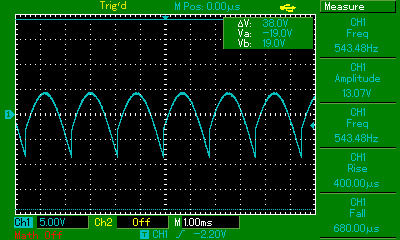
\includegraphics[width=\textwidth]{images/aufg2_phi0.jpg}
        \caption{Phase = $\SI{0}{\degree}$ ohne Störung}
        \label{fig:3a}
    \end{subfigure}
    \begin{subfigure}{0.495\linewidth}
        \centering
        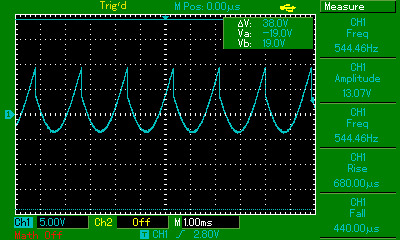
\includegraphics[width=\textwidth]{images/aufg3_phi0.jpg}
        \caption{Phase = $\SI{0}{\degree}$ mit Störung}
        \label{fig:3b}
    \end{subfigure}
    \begin{subfigure}{0.495\linewidth} % Phi = 90 --------------------------------------------------------------------------
        \centering
        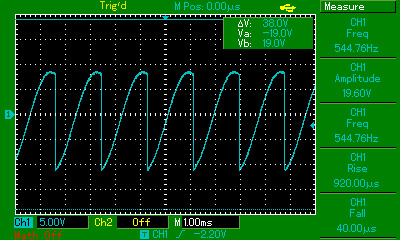
\includegraphics[width=\textwidth]{images/aufg2_phi90.jpg}
        \caption{Phase = $\SI{90}{\degree}$ ohne Störung}
        \label{fig:3c}
    \end{subfigure}
    \begin{subfigure}{0.495\linewidth}
        \centering
        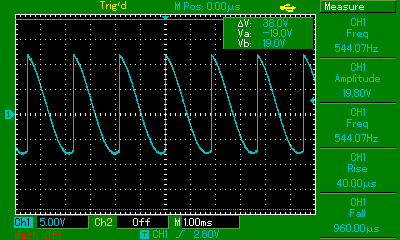
\includegraphics[width=\textwidth]{images/aufg3_phi90.jpg}
        \caption{Phase = $\SI{90}{\degree}$ mit Störung}
        \label{fig:3d}
    \end{subfigure}
    \begin{subfigure}{0.495\linewidth} % Phi = 135 --------------------------------------------------------------------------
        \centering
        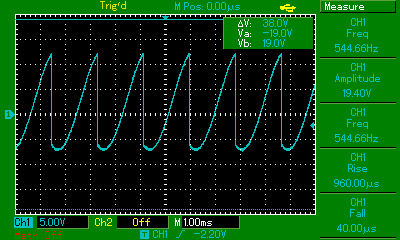
\includegraphics[width=\textwidth]{images/aufg2_phi135.jpg}
        \caption{Phase = $\SI{135}{\degree}$ ohne Störung}
        \label{fig:3e}
    \end{subfigure}
    \begin{subfigure}{0.495\linewidth}
        \centering
        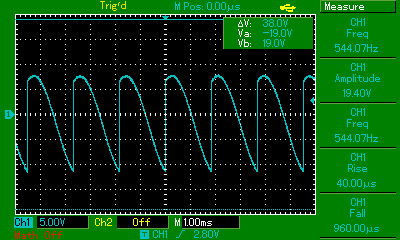
\includegraphics[width=\textwidth]{images/aufg3_phi135.jpg}
        \caption{Phase = $\SI{135}{\degree}$ mit Störung}
        \label{fig:3f}
    \end{subfigure}
    \begin{subfigure}{0.495\linewidth} % Phi = 180 --------------------------------------------------------------------------
        \centering
        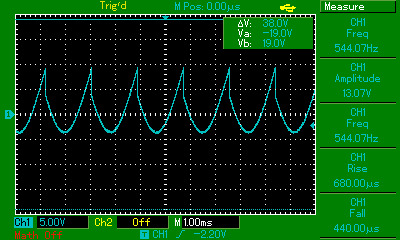
\includegraphics[width=\textwidth]{images/aufg2_phi180.jpg}
        \caption{Phase = $\SI{180}{\degree}$ ohne Störung}
        \label{fig:3g}
    \end{subfigure}
    \begin{subfigure}{0.495\linewidth}
        \centering
        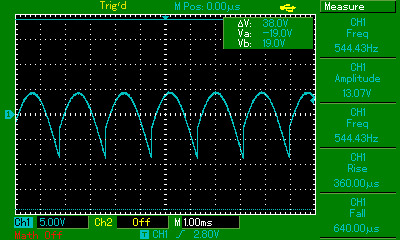
\includegraphics[width=\textwidth]{images/aufg3_phi180.jpg}
        \caption{Phase = $\SI{180}{\degree}$ mit Störung}
        \label{fig:3h}
    \end{subfigure}
    \begin{subfigure}{0.495\linewidth} % Phi = 270 --------------------------------------------------------------------------
        \centering
        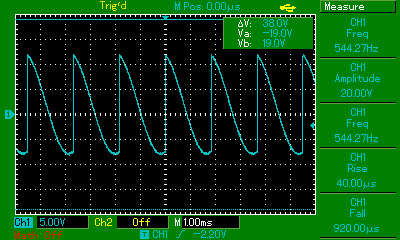
\includegraphics[width=\textwidth]{images/aufg2_phi270.jpg}
        \caption{Phase = $\SI{270}{\degree}$ ohne Störung}
        \label{fig:3i}
    \end{subfigure}
    \begin{subfigure}{0.495\linewidth}
        \centering
        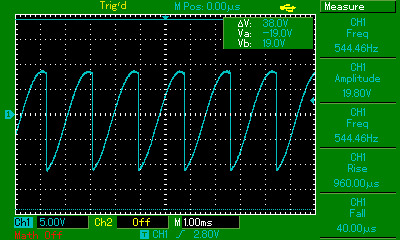
\includegraphics[width=\textwidth]{images/aufg3_phi270.jpg}
        \caption{Phase = $\SI{270}{\degree}$ mit Störung}
        \label{fig:3j}
    \end{subfigure}
\end{figure}

\begin{table}[H]
    \centering
    \input{table_oS.tex}
    \caption{Messwerte ohne Störung}
    \label{tab:1}
\end{table}

\begin{figure}[H]
    \centering
    \includegraphics[width=0.75\linewidth]{plotphi_oS.pdf}
    \caption{Nicht-lineare Regression des Signals ohne Störung}
    \label{fig:4}
\end{figure}

\begin{table}[H]
    \centering
    \input{table_mS.tex}
    \caption{Messwerte mit Störung}
    \label{tab:2}
\end{table}

\begin{figure}[H]
    \centering
    \includegraphics[width=0.75\linewidth]{plotphi_mS.pdf}
    \caption{Nicht-lineare Regression des Signals mit Störung}
    \label{fig:5}
\end{figure}

\begin{table}[H]
    \centering
    \input{table_I.tex}
    \caption{Messwerte der Intensität}
    \label{tab:3}
\end{table}

% Diskussion %%%%%%%%%%%%%%%%%%%%%%%%%%%%%%%%%%%%%%%%%%%%%%%%%%%%%%%%%%%%%%%%%%%%%%%%%%%%%%%%%%%%%%%%%%%%%%%%%%%%%%%%%%%%%%%%%%%%%%%%%%%%%%%%%%%%%%%%%%%%%%%%%%%%%%%%%%%%%%%%%%%%%%%%%%%%%%%%%%%%%%%%%%%%%%%%%%

\section{Diskussion}


% Literatur %%%%%%%%%%%%%%%%%%%%%%%%%%%%%%%%%%%%%%%%%%%%%%%%%%%%%%%%%%%%%%%%%%%%%%%%%%%%%%%%%%%%%%%%%%%%%%%%%%%%%%%%%%%%%%%%%%%%%%%%%%%%%%%%%%%%%%%%%%%%%%%%%%%%%%%%%%%%%%%%%%%%%%%%%%%%%%%%%%%%%%%%%%%%%%%%%%

\newpage
\printbibliography

\end{document}